\documentclass[12pt]{article}
\usepackage[utf8]{inputenc}
\usepackage[a4paper, margin=1in]{geometry}
\usepackage{graphicx}
\usepackage{tikz}
\usetikzlibrary{decorations.pathreplacing}
\usepackage{pgfplots}
\pgfplotsset{compat=1.18}
\usepackage{caption}
\usepackage{listings}
\usepackage{xcolor}
\usepackage{hyperref}
\usepackage{float}
\usepackage{booktabs}
\usepackage{makecell}

\definecolor{codegreen}{rgb}{0,0.6,0}
\definecolor{codegray}{rgb}{0.5,0.5,0.5}
\definecolor{codepurple}{rgb}{0.58,0,0.82}
\definecolor{backcolour}{rgb}{0.95,0.95,0.92}

\lstdefinestyle{mystyle}{
    backgroundcolor=\color{backcolour},   
    commentstyle=\color{codegreen},
    keywordstyle=\color{magenta},
    numberstyle=\tiny\color{codegray},
    stringstyle=\color{codepurple},
    basicstyle=\ttfamily\footnotesize,
    breakatwhitespace=false,         
    breaklines=true,                 
    captionpos=b,                    
    keepspaces=true,                 
    numbers=left,                    
    numbersep=5pt,                  
    showspaces=false,                
    showstringspaces=false,
    showtabs=false,                  
    tabsize=2
}
\lstset{style=mystyle}

\begin{document}

\begin{titlepage}
    \centering
    \vspace*{2cm}
    
    {\Large\bfseries Assignment 2: Implement Flow Control Mechanisms for Data Link Layer\par}
    \vspace{2cm}
    
    {\Large\bfseries Name: Aritra Dutta\par}
    \vspace{1cm}
    
    {\Large\bfseries Class: BCSE III\par}
    \vspace{1cm}
    
    {\Large\bfseries Roll: 002410501009\par}
    \vspace{1cm}
    
    {\Large\bfseries Group: A1\par}
    \vspace{1cm}
    
    {\Large\bfseries College: Jadavpur University\par}
    \vspace{1.5cm}
    
    {\normalsize\bfseries GitHub Repository: \url{https://github.com/Aricode2005/CN-LAB}\par}
    
    \vfill
\end{titlepage}

\tableofcontents
\newpage

\section{Introduction}
Modern communication networks rely on the Data Link Layer to ensure reliable data transfer over inherently unreliable physical channels. The Data Link Layer is classically divided into two sublayers: the Media Access Control (MAC) sublayer, which handles framing and physical addressing, and the Logical Link Control (LLC) sublayer, which manages multiplexing, flow control, and error recovery. 

While error detection schemes (such as the Cyclic Redundancy Check and Checksum algorithms explored in Assignment 1) allow a receiver to mathematically identify corrupted frames, they do not inherently recover lost data. To achieve true reliability, the LLC sublayer requires the implementation of \textbf{Flow Control} and \textbf{Automatic Repeat reQuest (ARQ)} mechanisms. Flow control prevents a fast sender from overwhelming a slow receiver, while ARQ ensures that any frame lost or corrupted in transit is automatically retransmitted until successfully acknowledged.

In this assignment, we design and implement three fundamental flow control mechanisms: Stop-and-Wait ARQ, Go-Back-N (GBN) ARQ, and Selective Repeat (SR) ARQ. The entire system is simulated using a client-server architecture via Java TCP sockets. To simulate the chaotic nature of physical network mediums, we artificially incorporate probabilistic network latency and bit-level corruption. This allows us to rigorously evaluate how these protocols respond to frame loss, sequence wrap-arounds, and dynamic network timeouts under stress.

\subsection{Data Frame Structure}
Following the IEEE 802.3 Ethernet standard, our simulated frames carry a minimum payload, encapsulated with a MAC header, length, sequence number, and a Frame Check Sequence (FCS) trailer. A dedicated 1-byte field is assigned for the \textbf{Sequence Number}, which acts as the mathematical backbone for the logical flow control of the ARQ protocols.

\begin{figure}[H]
    \centering
    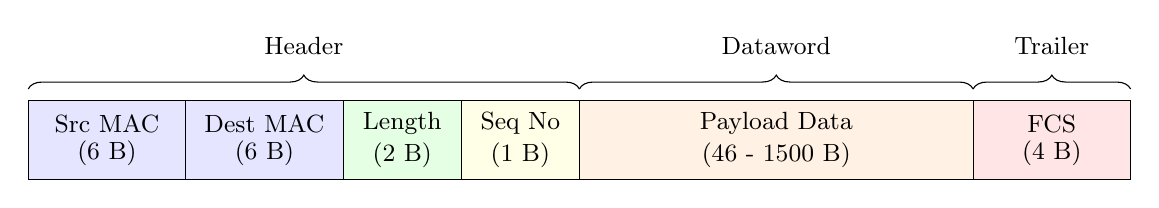
\begin{tikzpicture}[font=\small, text centered]
    % Header
    \draw[fill=blue!10] (0,0) rectangle (2,1) node[midway] {\shortstack{Src MAC \\ (6 B)}};
    \draw[fill=blue!10] (2,0) rectangle (4,1) node[midway] {\shortstack{Dest MAC \\ (6 B)}};
    \draw[fill=green!10] (4,0) rectangle (5.5,1) node[midway] {\shortstack{Length \\ (2 B)}};
    \draw[fill=yellow!10] (5.5,0) rectangle (7,1) node[midway] {\shortstack{Seq No \\ (1 B)}};
    
    % Payload
    \draw[fill=orange!10] (7,0) rectangle (12,1) node[midway] {\shortstack{Payload Data \\ (46 - 1500 B)}};
    
    % Trailer
    \draw[fill=red!10] (12,0) rectangle (14,1) node[midway] {\shortstack{FCS \\ (4 B)}};
    
    % Braces
    \draw [decorate,decoration={brace,amplitude=5pt,raise=1ex}] 
      (0,1) -- (7,1) node[midway,yshift=2em] {Header};
    \draw [decorate,decoration={brace,amplitude=5pt,raise=1ex}] 
      (7,1) -- (12,1) node[midway,yshift=2em] {Dataword};
    \draw [decorate,decoration={brace,amplitude=5pt,raise=1ex}] 
      (12,1) -- (14,1) node[midway,yshift=2em] {Trailer};
    \end{tikzpicture}
    \caption{Simulated Data Link Layer Frame Structure}
\end{figure}

The inclusion of the sequence number allows the Receiver to track order, discard duplicates, and request specific retransmissions, which forms the core behavioral logic of GBN and SR.

\section{Problem Statement}
The objective is to design and implement flow control mechanisms of the Logical Link Control (LLC) sublayer within a simulated network environment. 

The \textbf{Sender Program} must consist of the following methods:
\begin{itemize}
    \item \textbf{Framing()}: Prepares the frame with a header (MAC addresses, Length, Frame Sequence Number), a 46-1500 byte payload read from a text file, and a 4-byte CRC/Checksum FCS trailer calculated from the Assignment 1 module.
    \item \textbf{Channel()}: Introduces random probabilistic delay (causing packet loss or extreme timeout) and/or bit errors using the error injection module while transferring frames to the receiver.
    \item \textbf{Send()}: Transmits data frames via socket connection to the Receiver program. The Sender must autonomously decide whether to send new data frames or retransmit old frames due to timeout expirations.
    \item \textbf{Timer()}: A timer must be associated with each frame transmission to strictly monitor the timeout condition.
    \item \textbf{Timeout()}: Computes the most recent data frame's Round-Trip Time (RTT) to dynamically re-compute and adjust the value of the network timeout.
    \item \textbf{Recv()}: Invoked by the Sender program whenever an ACK packet is returned. It considers network time when the ACK was received to update sliding windows and cancel associated timers.
\end{itemize}

The \textbf{Receiver Program} must independently implement the following:
\begin{itemize}
    \item \textbf{Recv()}: Invoked continuously whenever a Data frame arrives from the network.
    \item \textbf{Check()}: Verifies data integrity using the CRC/Checksum FCS. Discards the frame silently if a bit-error is detected.
    \item \textbf{Send()}: Prepares and transmits an acknowledgement frame (ACK/NAK) containing the expected sequence number, sending it back to the sender as a response to successful receipt.
\end{itemize}

The system must implement \textbf{Stop-and-Wait}, \textbf{Go-Back-N (GBN)}, and \textbf{Selective Repeat (SR)}, and strictly evaluate their comparative efficiency and propagation latency under varying probabilities (0.1 to 0.5) of error and delay.

\section{System Architecture and Methodology}
The software architecture is developed in Java, utilizing multithreaded POSIX-style Socket Programming. To successfully simulate an unreliable physical layer (like a noisy Ethernet cable or wireless signal) over a perfectly reliable TCP socket, we implemented a custom \texttt{NetworkSimulator} middleware.

\subsection{Multithreading and Synchronization}
Because network packets can arrive at any arbitrary millisecond, the application requires parallel execution. The architecture relies on three tightly choreographed threads managed through Java's Wait/Notify synchronization paradigm on an intrinsic intrinsic \texttt{lock} monitor:
\begin{enumerate}
    \item \textbf{The Main Thread (Transmitter):} Executes the \texttt{Send()} method. It slices the file into frames, pushes them onto the physical wire, and calls \texttt{lock.wait()} to willingly put itself to sleep while waiting for an ACK.
    \item \textbf{The Listener Thread (Receiver Engine):} A background \texttt{Thread} running an infinite \texttt{socket.receive()} loop. When it hears an ACK arrive, it temporarily grabs the \texttt{lock}, updates the window sliding variables safely, and yells \texttt{lock.notifyAll()} to instantaneously wake up the sleeping Main Thread.
    \item \textbf{The Timer Thread (Alarm Clock):} Managed by \texttt{java.util.Timer}. If a timer expires before an ACK arrives, this thread grabs the \texttt{lock}, resets the window pointers to trigger a retransmission, and calls \texttt{notifyAll()} to wake the Main Thread.
\end{enumerate}

\subsection{Sequence Number Space and Modulo Arithmetic}
In physical network hardware, frame headers are strictly limited by bit-size. For this implementation, the sequence number bit-size ($m$) is fixed to \textbf{4 bits}. This yields a maximum sequence space of $2^4 = 16$, meaning the physical sequence numbers stamped on the frames cycle exclusively from 0 through 15. 

Both the Sender and Receiver maintain absolute integer indices logically in memory to track their position in the file, but they intentionally wrap the physical sequence numbers inside the frame headers using modulo arithmetic: \texttt{seqNo \% 16}. This accurately simulates the hardware limitation and forces the ARQ protocols to deal with the complexities of sequence wrap-around math.

\subsection{The Network Simulator and Deep-Clone Error Injection}
The \texttt{NetworkSimulator} intercepts every frame before it hits the socket. Based on the user-defined \texttt{errorProbability} and \texttt{delayProbability}, it executes two completely independent probabilistic dice rolls:

A critical architectural challenge in Java is that objects are passed by reference. If the simulator mutates the \texttt{Frame} object directly, it will corrupt the Sender's local memory buffer, meaning any subsequent retransmissions would be permanently broken. To solve this, the simulator utilizes \textbf{Deep Cloning via Object Serialization} to create a detached, disposable replica of the frame. It injects the bit-errors exclusively into the clone, preserving the integrity of the Sender's original frame memory.

\begin{lstlisting}[language=Java, caption=NetworkSimulator Independent Dice Rolls]
public void sendWithSimulation(...) throws IOException {
    // 1. Deep Clone via Serialization to protect Sender's physical memory
    byte[] data = serialize(obj);
    
    // 2. ERROR DICE ROLL: Inject Bit-Errors probabilistically
    if (!isRetransmission && random.nextDouble() < errorProbability) {
        Object clonedObj = deserialize(data);
        errorInjector.execute(((Frame) clonedObj).getPayload()); // Flip bits
        data = serialize(clonedObj); // Repackage corrupted frame
    }
    
    // 3. DELAY DICE ROLL: Inject Network Latency (Thread sleep)
    int delay = 0;
    if (!isRetransmission && random.nextDouble() < delayProbability) {
        delay = maxDelayMs + random.nextInt(2000); // Massive delay up to 2.01 seconds
        Thread.sleep(delay);
    }
    
    // 4. Transmit over Socket
    socket.send(new DatagramPacket(data, data.length, address, port));
}
\end{lstlisting}
*(Note: As a smart design choice, if the simulator detects that a packet is a \texttt{isRetransmission}, it bypasses both dice rolls to prevent the simulation from trapping the protocol in an infinite loop of bad luck).*

\subsection{Simulating Packet Loss via Extreme Latency}
Rather than simply deleting \texttt{Frame} objects from memory, this implementation takes a highly realistic approach to packet loss: \textbf{Extreme Latency}. Right before the Sender pushes a frame onto the physical wire, it explicitly stamps it with the absolute current clock time (\texttt{System.currentTimeMillis()}).
When the Receiver gets the frame, it calculates the transit delta. If the delta is greater than a strict \texttt{MAX\_LIFETIME} (set to 2500 ms), the Receiver realizes the packet was trapped in a slow router by the simulator. The Receiver actively throws the old packet in the trash, successfully simulating a true packet drop and forcing the Sender's timer to expire.

\section{Protocol Implementations}

\subsection{Stop-and-Wait ARQ}
Stop-and-Wait is the most rudimentary flow control mechanism. The sender transmits exactly one frame and completely halts execution, waiting for an ACK before proceeding. The sequence number alternates exclusively between 0 and 1 ($m=1$). 

The \texttt{Send} loop acts as a \textbf{Retransmission Loop}. By setting \texttt{waitingForAck = true} before the loop, we guarantee it enters the block. It transmits the frame and then puts the Main Thread to sleep via \texttt{lock.wait()}. If the timer expires, the thread wakes up, hits the bottom of the loop, and goes back to the top. Because \texttt{waitingForAck} is still true, the loop repeats, actively retransmitting the exact same frame!

\begin{lstlisting}[language=Java, caption=Stop-and-Wait Retransmission Loop]
public void Send(byte[][] dataChunks) throws Exception {
    for (byte[] data : dataChunks) {
        seqNo = (seqNo + 1) % 2; // Sequence number strictly alternates 0, 1, 0, 1
        currentFrame = Framing(seqNo, data);
        
        waitingForAck = true;
        while (waitingForAck) {  // The Retransmission Loop
            Channel(currentFrame); // Send the frame
            Timer(seqNo);          // Start the clock
            
            synchronized (lock) {
                lock.wait(currentTimeoutMs); // The algorithm STOPS and WAITS right here.
            }
        }
    }
}
\end{lstlisting}

When a valid ACK finally arrives at the Listener Thread, the background thread forces the `while` condition to become false and explicitly wakes up the Main Thread, terminating the retransmission cycle.
\begin{lstlisting}[language=Java, caption=Stop-and-Wait Success Notification]
protected void Recv(Ack ack) {
    if (ack.getAckNo() == (seqNo + 1) % 2) { 
        waitingForAck = false; // Break the Retransmission Loop
        lock.notifyAll(); // Wake up the sleeping Main Thread
    }
}
\end{lstlisting}

\subsection{Go-Back-N (GBN) ARQ}
Go-Back-N dramatically improves channel utilization by employing a \textbf{Sliding Window} of size $N$. The sender pipelines up to $N$ unacknowledged frames into the network consecutively. 

\subsubsection{Strict Reception and Cumulative ACKs}
The Receiver window is strictly `1`, meaning it refuses out-of-order packets. It expects packets sequentially. If it gets Frame 0, it asks for Frame 1 by sending \texttt{ACK 1}. If it receives Frame 3 instead of 1, it drops Frame 3 and stubbornly sends \texttt{ACK 1} again.

On the Sender side, ACKs are interpreted \textbf{Cumulatively}. If the Sender receives \texttt{ACK 4}, the mathematical logic inherently verifies that Frames 0, 1, 2, and 3 must have all been successfully received (even if the individual ACKs for 0, 1, and 2 were utterly destroyed in transit). The sender instantly slides its base to 4.

\begin{lstlisting}[language=Java, caption=Go-Back-N Sender Cumulative ACK Logic]
protected void Recv(Ack ack) {
    int ackNo = ack.getAckNo();
    int absAckNo = getAbsoluteAck(ackNo, base); // Solve Modulo wrap-around
    
    // CUMULATIVE LOGIC: Any valid ACK slides the window covering all prior frames
    if (absAckNo > base && absAckNo <= nextSeqNum) {
        Timeout(); // Calculate dynamic RTT
        base = absAckNo; // Slide the base forward!
        lock.notifyAll();
    }
}
\end{lstlisting}

\subsubsection{The Modulo Mapping Problem}
Because physical sequence numbers wrap from 15 back to 0, if the sender receives an \texttt{ACK 2}, it doesn't know if that means logical array index 2, 18, or 34. To slide the window, we must dynamically calculate the \textit{Absolute Sequence Number} based on where the current window is resting.

\begin{lstlisting}[language=Java, caption=Resolving Sequence Wrap-Around]
private int getAbsoluteAck(int ackNo, int base) {
    int baseMod = base % Frame.MAX_SEQ;
    int diff = ackNo - baseMod;
    if (diff <= 0) diff += Frame.MAX_SEQ; // Calculate forward wrapping difference
    
    int abs = base + diff;
    if (abs > base + windowSize) {
        abs -= Frame.MAX_SEQ; // Ignore ancient, erroneously delayed ACKs
    }
    return abs;
}
\end{lstlisting}

\subsubsection{The Timeout Punishment}
If a timeout occurs at the sender, it assumes all unacknowledged frames were lost. The Timer Thread ruthlessly resets the transmission pointer (\texttt{nextSeqNum}) all the way back to the oldest unacknowledged frame (\texttt{base}). When the Main Thread wakes up, its loop condition immediately begins retransmitting the entire window from scratch.

\begin{lstlisting}[language=Java, caption=Go-Back-N Timeout Punishment]
protected void handleTimeout(int seqNo) {
    if (seqNo == base % Frame.MAX_SEQ) {
        // Reset the transmission pointer all the way back to the base
        nextSeqNum = base; 
        lock.notifyAll(); // Main Thread wakes up and resends entire window
    }
}
\end{lstlisting}

\subsection{Selective Repeat (SR) ARQ}
Selective Repeat maximizes theoretical efficiency on noisy channels by decoupling the sender and receiver windows. The receiver utilizes a window size of $N$ and maintains an internal buffer (using a Java \texttt{HashMap}) to accept and temporarily store out-of-order frames.

\subsubsection{Independent Timers and NAKs}
Unlike GBN, which only times the oldest frame, the SR Sender starts an **Independent Timer** for every single frame. If the Receiver detects a corrupted frame, it immediately fires back an explicit **NAK** (Negative Acknowledgement). The Sender bypasses the timer entirely, performing a surgical strike to retransmit only the broken frame.

\begin{lstlisting}[language=Java, caption=Selective Repeat Receiver NAK and Buffering]
// Inside SelectiveRepeatReceiver.java
if (!Check(frame)) {
    Send(seqNo, true); // Send explicit NAK (true = isNak)
    return;
}

// Out-Of-Order Buffering Logic
if (seqNo >= base && seqNo < base + windowSize) {
    buffer.put(seqNo, frame); // Save out-of-order frame in memory
    Send(seqNo, false);       // Send Independent ACK

    // Slide window forward ONLY if the base contiguous frame arrived
    while (buffer.containsKey(base)) {
        deliverDataToApplication(buffer.remove(base).getPayload());
        base++;
    }
}
\end{lstlisting}

\subsubsection{The "Ghost Frame" Re-ACKing Rule}
A critical edge-case occurs when the Receiver successfully processes Frame 0 and sends \texttt{ACK 0}, but \texttt{ACK 0} gets lost in the network. The Sender's timer for Frame 0 will eventually expire, and the Sender will redundantly retransmit Frame 0. When that old Frame 0 hits the Receiver, it falls \textit{behind} the Receiver's current window. If the Receiver ignores it, the Sender will be trapped waiting forever. Thus, the Receiver must actively re-ACK old duplicates to rescue the stuck Sender.

\begin{lstlisting}[language=Java, caption=Selective Repeat Ghost Frame Rescue]
// If the frame sequence is older than our current base window...
} else if (seqNo >= base - windowSize && seqNo < base) {
    // Send a duplicate ACK so the Sender's expired timer stops!
    Send(seqNo, false); 
}
\end{lstlisting}


\section{Experimental Evaluation and Results}
To scientifically evaluate the protocols, an automated \texttt{TestRunner} was executed under a 30-frame payload transmission. 
\textbf{Efficiency} is calculated as the ratio of actual original application frames to the total number of frames physically transmitted across the network (including all redundant retransmissions). The formula is strictly $\frac{Original}{Total Transmitted} \times 100$.

\subsection{Base Case (0\% Error, 0\% Delay)}
Under perfect, ideal network conditions (no interference), pipelined protocols vastly outperform Stop-and-Wait, approaching 100\% efficiency. By calculating the difference between the frame timestamp and ACK reception time, we observe that Stop-and-Wait suffers the worst Average Round-Trip Time (RTT) because it sits completely idle between frames, whereas pipelined protocols aggressively overlap their propagation times.

\begin{table}[H]
\centering
\begin{tabular}{@{}lcccc@{}}
\toprule
\textbf{Protocol} & \textbf{Window Size} & \textbf{Efficiency} & \textbf{Avg RTT} & \textbf{Total Time} \\ \midrule
Stop-and-Wait     & 1                  & 96.8\%              & 9 ms             & 445 ms              \\
Go-Back-N         & 7                  & 100.0\%             & 4 ms             & 239 ms              \\
Selective Repeat  & 7                  & 100.0\%             & 1 ms             & 246 ms              \\ \bottomrule
\end{tabular}
\caption{Base Case Transmission Metrics}
\end{table}

\subsection{Efficiency vs. Error Probability}
As the bit-error probability increases (with delay held constant at 0\%), the structural weaknesses of Stop-and-Wait and GBN become glaringly apparent. Stop-and-Wait's execution time spirals out of control due to sequential bottlenecks. Go-Back-N suffers severe efficiency penalties because a single bit-error forces the wasteful retransmission of the entire window, clogging the network with redundant data. Selective Repeat maintains the highest efficiency by surgically retransmitting only the corrupted frames.

\begin{table}[H]
\centering
\begin{tabular}{@{}lccccc@{}}
\toprule
\textbf{Protocol} & \textbf{0.1} & \textbf{0.2} & \textbf{0.3} & \textbf{0.4} & \textbf{0.5} \\ \midrule
Stop-and-Wait     & 83.3\% & 76.9\% & 52.6\% & 52.6\% & 41.1\% \\
Go-Back-N         & 68.2\% & 61.2\% & 56.6\% & 54.5\% & 51.7\% \\
Selective Repeat  & 81.1\% & 68.2\% & 58.8\% & 51.7\% & 37.0\% \\ \bottomrule
\end{tabular}
\caption{Efficiency under varying Error Probabilities}
\end{table}

\begin{figure}[H]
    \centering
    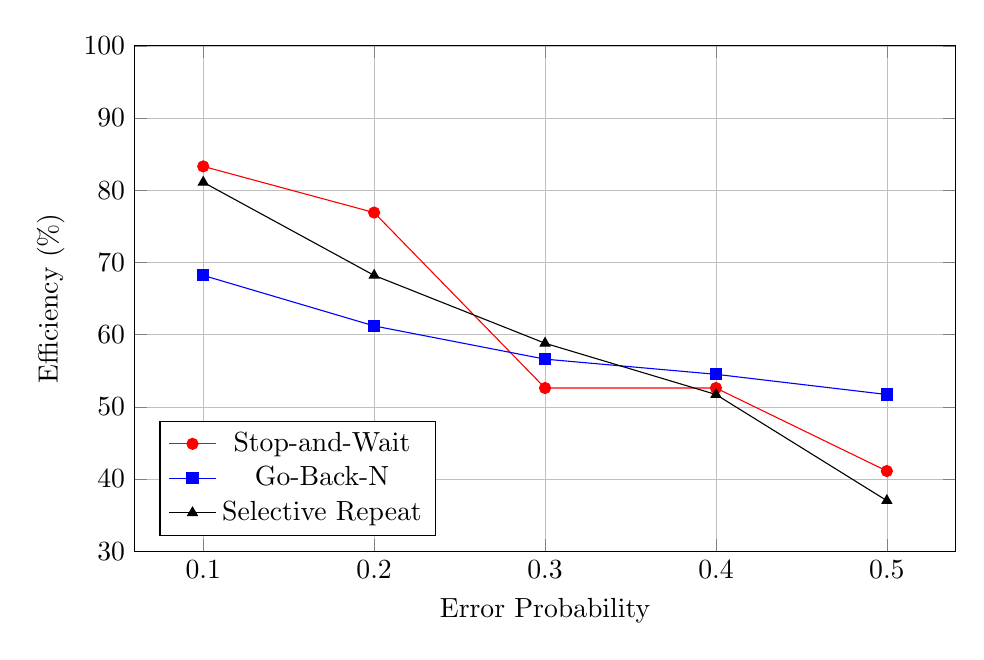
\begin{tikzpicture}
    \begin{axis}[
        width=12cm, height=8cm,
        xlabel={Error Probability},
        ylabel={Efficiency (\%)},
        ymin=30, ymax=100,
        xtick={0.1, 0.2, 0.3, 0.4, 0.5},
        legend pos=south west,
        grid=both,
        grid style={line width=.1pt, draw=gray!30},
        major grid style={line width=.2pt,draw=gray!50}
    ]
    \addplot[color=red, mark=*] coordinates {
        (0.1, 83.3) (0.2, 76.9) (0.3, 52.6) (0.4, 52.6) (0.5, 41.1)
    };
    \addplot[color=blue, mark=square*] coordinates {
        (0.1, 68.2) (0.2, 61.2) (0.3, 56.6) (0.4, 54.5) (0.5, 51.7)
    };
    \addplot[color=black, mark=triangle*] coordinates {
        (0.1, 81.1) (0.2, 68.2) (0.3, 58.8) (0.4, 51.7) (0.5, 37.0)
    };
    \legend{Stop-and-Wait, Go-Back-N, Selective Repeat}
    \end{axis}
    \end{tikzpicture}
    \caption{Protocol Efficiency as Error Probability Scales}
\end{figure}

\subsection{Efficiency vs. Delay Probability}
Delay probability causes packets to exceed the receiver's \texttt{MAX\_LIFETIME}, triggering sender timeouts. Selective Repeat handles random delays exceptionally well due to its independent timers and out-of-order buffering. Go-Back-N performs terribly under high delay because, while the receiver discards the delayed packet, it also discards all subsequent, perfectly valid packets in the window, forcing massive cumulative retransmissions.

\begin{table}[H]
\centering
\begin{tabular}{@{}lccccc@{}}
\toprule
\textbf{Protocol} & \textbf{0.1} & \textbf{0.2} & \textbf{0.3} & \textbf{0.4} & \textbf{0.5} \\ \midrule
Stop-and-Wait     & 81.1\% & 83.3\% & 83.3\% & 83.3\% & 85.7\% \\
Go-Back-N         & 41.7\% & 41.7\% & 55.6\% & 46.2\% & 50.0\% \\
Selective Repeat  & 63.8\% & 66.7\% & 73.2\% & 62.5\% & 69.8\% \\ \bottomrule
\end{tabular}
\caption{Efficiency under varying Delay Probabilities}
\end{table}

\begin{figure}[H]
    \centering
    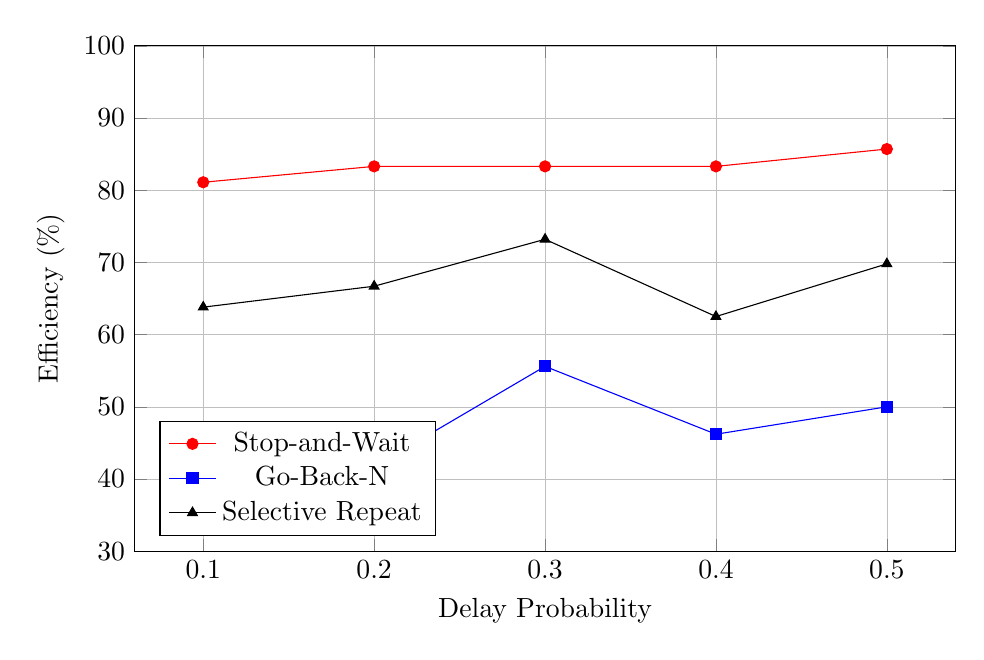
\begin{tikzpicture}
    \begin{axis}[
        width=12cm, height=8cm,
        xlabel={Delay Probability},
        ylabel={Efficiency (\%)},
        ymin=30, ymax=100,
        xtick={0.1, 0.2, 0.3, 0.4, 0.5},
        legend pos=south west,
        grid=both,
        grid style={line width=.1pt, draw=gray!30},
        major grid style={line width=.2pt,draw=gray!50}
    ]
    \addplot[color=red, mark=*] coordinates {
        (0.1, 81.1) (0.2, 83.3) (0.3, 83.3) (0.4, 83.3) (0.5, 85.7)
    };
    \addplot[color=blue, mark=square*] coordinates {
        (0.1, 41.7) (0.2, 41.7) (0.3, 55.6) (0.4, 46.2) (0.5, 50.0)
    };
    \addplot[color=black, mark=triangle*] coordinates {
        (0.1, 63.8) (0.2, 66.7) (0.3, 73.2) (0.4, 62.5) (0.5, 69.8)
    };
    \legend{Stop-and-Wait, Go-Back-N, Selective Repeat}
    \end{axis}
    \end{tikzpicture}
    \caption{Protocol Efficiency as Delay Probability Scales}
\end{figure}

\section{Window Size Analysis}
To mathematically evaluate the impact of window size ($N$) on performance, a dedicated analyzer script recorded the efficiency and Average RTT as the window scaled. The tests were run with a static 10\% delay probability to induce natural retransmissions.

\begin{table}[H]
\centering
\begin{tabular}{@{}lcccc@{}}
\toprule
\textbf{Protocol} & \textbf{Window Size (N)} & \textbf{Efficiency (\%)} & \textbf{Avg RTT (ms)} \\ \midrule
GBN               & 2                      & 83.3\%                   & 157 ms              \\
GBN               & 4                      & 71.4\%                   & 98 ms               \\
GBN               & 8                      & 78.9\%                   & 142 ms              \\
GBN               & 12                     & 71.4\%                   & 360 ms              \\
GBN               & 15                     & 66.7\%                   & 80 ms               \\ \midrule
SR                & 2                      & 93.8\%                   & 2 ms                \\
SR                & 4                      & 81.1\%                   & 2 ms                \\
SR                & 6                      & 85.7\%                   & 3 ms                \\
SR                & 8                      & 81.1\%                   & 3 ms                \\ \bottomrule
\end{tabular}
\caption{Window Size vs. Throughput Metrics}
\end{table}

\begin{figure}[H]
    \centering
    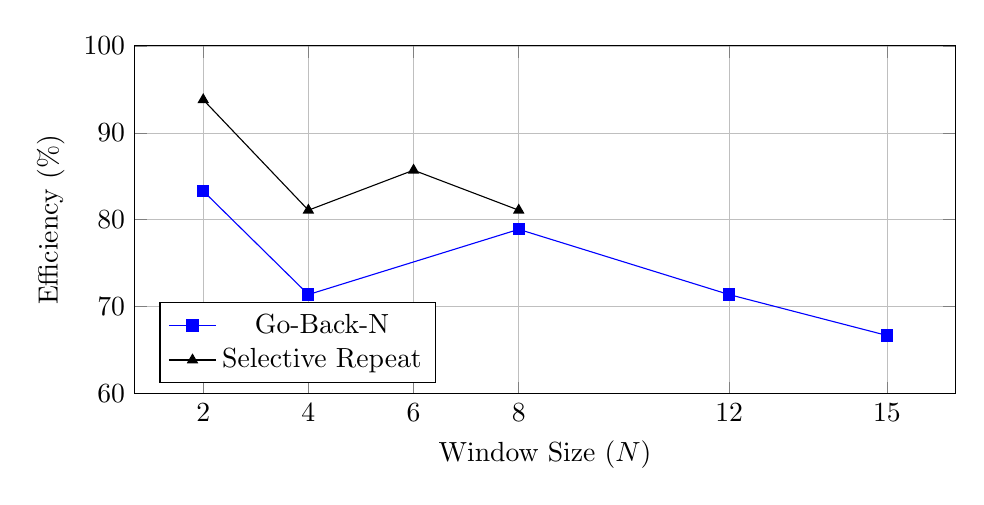
\begin{tikzpicture}
    \begin{axis}[
        width=12cm, height=6cm,
        xlabel={Window Size ($N$)},
        ylabel={Efficiency (\%)},
        ymin=60, ymax=100,
        xtick={2, 4, 6, 8, 12, 15},
        legend pos=south west,
        grid=both,
        grid style={line width=.1pt, draw=gray!30},
        major grid style={line width=.2pt,draw=gray!50}
    ]
    \addplot[color=blue, mark=square*] coordinates {
        (2, 83.3) (4, 71.4) (8, 78.9) (12, 71.4) (15, 66.7)
    };
    \addplot[color=black, mark=triangle*] coordinates {
        (2, 93.8) (4, 81.1) (6, 85.7) (8, 81.1)
    };
    \legend{Go-Back-N, Selective Repeat}
    \end{axis}
    \end{tikzpicture}
    \caption{Protocol Efficiency as Window Size Scales}
\end{figure}

\begin{figure}[H]
    \centering
    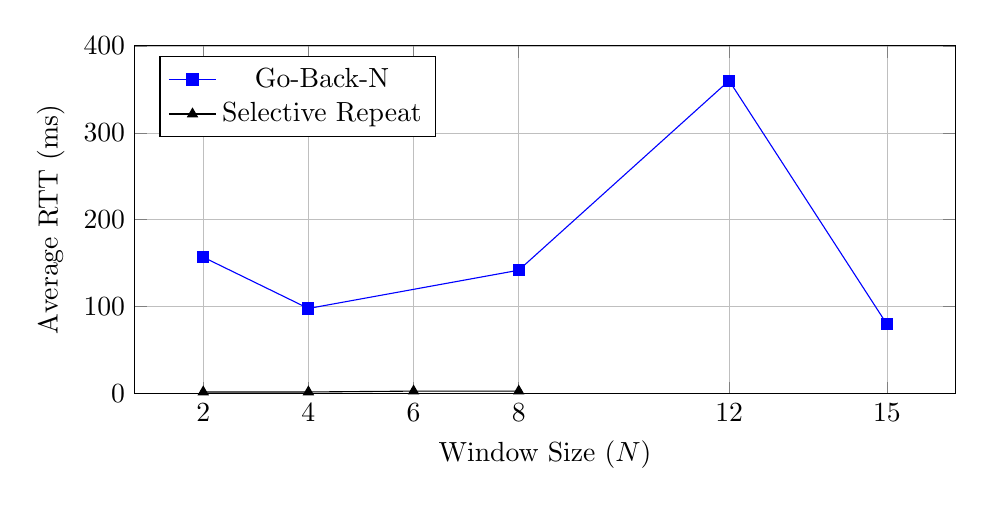
\begin{tikzpicture}
    \begin{axis}[
        width=12cm, height=6cm,
        xlabel={Window Size ($N$)},
        ylabel={Average RTT (ms)},
        ymin=0, ymax=400,
        xtick={2, 4, 6, 8, 12, 15},
        legend pos=north west,
        grid=both,
        grid style={line width=.1pt, draw=gray!30},
        major grid style={line width=.2pt,draw=gray!50}
    ]
    \addplot[color=blue, mark=square*] coordinates {
        (2, 157) (4, 98) (8, 142) (12, 360) (15, 80)
    };
    \addplot[color=black, mark=triangle*] coordinates {
        (2, 2) (4, 2) (6, 3) (8, 3)
    };
    \legend{Go-Back-N, Selective Repeat}
    \end{axis}
    \end{tikzpicture}
    \caption{Average RTT as Window Size Scales}
\end{figure}

The empirical data demonstrates a counter-intuitive principle: for Go-Back-N, expanding the window size actually \textit{decreases} efficiency and creates massive RTT spikes on noisy channels. This is because a larger window means more frames are pipelined into the network; when a single error occurs, the massive number of pipelined frames are all subsequently discarded and must be retransmitted, creating a severe penalty. Selective Repeat avoids this penalty, maintaining flat RTTs and robust efficiency regardless of how large the window scales.

\section{Window Failures and Mathematical Limits}
ARQ protocols mathematically depend on the sequence number space ($2^m$). The sequence numbers embedded in the physical frames act as the only logical compass the receiver has. If the sender's window size ($N$) violates strict mathematical boundaries relative to the sequence space, severe logic errors occur at the Data Link Layer, specifically resulting in the \textbf{Erroneous Acceptance} of old, delayed packets.

For a 4-bit sequence space ($2^4 = 16$), the physical sequence numbers wrap around from 15 back to 0. The Java simulation empirically verified the following theoretical failure states:

\subsection{Go-Back-N Failure Case ($N \ge 2^m$)}
When the window size is set to $N = 16$, the transmission window perfectly overlaps the entire sequence space. If Frame 0 is severely delayed by the network (e.g., trapped in a slow router), the sender eventually times out and re-sends the entire window (Frames 0 through 15). The receiver successfully accepts the retransmitted window, advances its expected sequence number across the entire space, and wraps around back to expecting Frame 0. 

When the original, severely delayed Frame 0 finally emerges from the slow router and arrives at the destination, it possesses the exact sequence number (0) that the receiver is currently expecting for the \textit{next} cycle. The receiver erroneously accepts this ancient duplicate, permanently corrupting the data stream. Thus, to ensure the receiver's window and the sender's retransmission window can never ambiguously overlap on a wrap-around, GBN strictly requires $N \le 2^m - 1$.

\subsection{Selective Repeat Failure Case ($N > 2^{m-1}$)}
Selective Repeat requires an even stricter boundary: $N \le 2^{m-1}$ (which means $N \le 8$ in our 4-bit simulation). Because the Selective Repeat receiver actively buffers out-of-order packets, its acceptance window spans multiple sequence numbers simultaneously. 

If $N = 9$, the sender's transmission window and the receiver's out-of-order acceptance window can overlap across the sequence space's wrap-around boundary. If an ACK for Frame 0 is lost, the sender's window halts waiting for it. However, the receiver successfully got the frame, so its acceptance window slides forward, wrapping around to logically include the \textit{next cycle's} Frame 0. When the sender's timer expires, it retransmits the old Frame 0. The receiver captures it, sees that Sequence 0 is currently a valid slot in its forward-shifted buffer, and accepts it, mistakenly believing it is the new Frame 0 of the next payload segment. This completely desynchronizes the payload assembly. Therefore, SR windows can never exceed half the sequence space.

\section{Conclusion}
This assignment successfully simulated and rigorously analyzed Data Link Layer flow control using multithreaded Java sockets. Stop-and-Wait provides absolute reliability but suffers from terrible bandwidth utilization, making it unviable for long-distance networks. Go-Back-N efficiently pipelines data but suffers catastrophic efficiency drops on noisy channels due to its reliance on cumulative retransmissions. Selective Repeat emerged as the mathematically and practically superior protocol, minimizing retransmissions through independent buffering and surgical fault recovery, provided its window size is strictly restricted to half the sequence space to prevent wrapping collisions.

\end{document}